\documentclass{beamer}
\usetheme{metropolis} 
\usepackage{caption}
\usepackage[utf8]{inputenc}


\title{\huge Konobi}
\date{}
\subtitle{Software Development Methods project}
\author{Lorenzo Basile, Irene Brugnara, Roberto Corti, Arianna Tasciotti}

\begin{document}
	
  \maketitle
  \section{Introduction}
  
  \begin{frame}{Our project}
    The goal of our project was to develop a command line version of \textbf{Konobi}, a board game for two players. The project also contains a client-server version of the game, which allows the two players to play remotely.
    \vspace{0.7cm}
    \pause
    \\What tools did we use?
    \begin{itemize}
	    \item Java 15
	    \item Gradle
	    \item TravisCI
	    \item Git \& GitHub
    \end{itemize}

  \end{frame}
  
  \begin{frame}{Konobi}
	    Konobi is a drawless game and it can be played either on a go board or a chess board.
	    \\Two players, black and white, take turns at placing stones of their color on the board, starting with black. The aim of the players is to build chains of connected stones of their color.
	    \vspace{0.5cm}
	    \pause
	    \\The game is won by the first player who connects the two opposite edges of the board.
	    \begin{itemize}
	    \item Black: top $\leftrightarrow$ bottom
	    \item White: left $\leftrightarrow$ right
	    \end{itemize}
   \end{frame}
      
   \begin{frame}{Connections}
     Two like-colored stones can be:
     \vspace{0.5cm}
    \begin{columns}
			\column{0.5\textwidth}
			\begin{figure}
				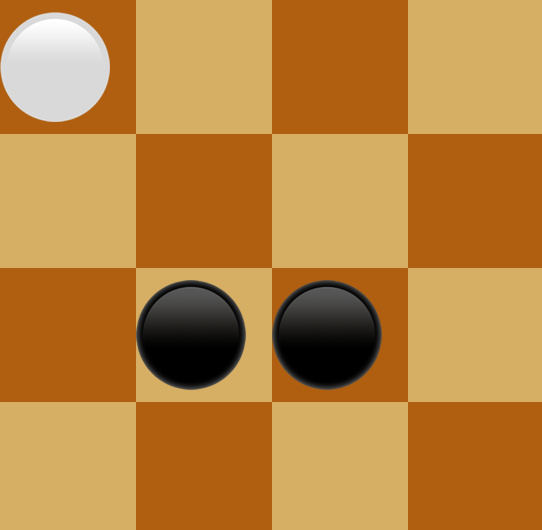
\includegraphics[scale=0.35]{images/strong.png}
				\caption*{Strongly connected}
			\end{figure}
					
			\column{0.5\textwidth}
			\begin{figure}
				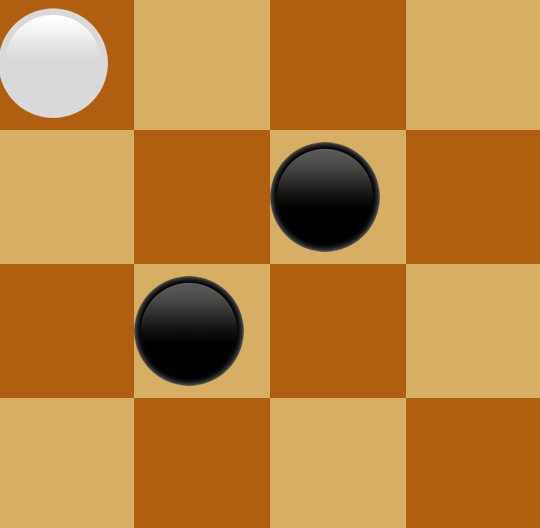
\includegraphics[scale=0.35]{images/weak.png}
				\caption*{Weakly connected}
			\end{figure}
		
	\end{columns}
	\vspace{0.7cm}
	A chain is a set of connected stones

      \end{frame}
      
      \begin{frame}{Placement rules}
     Not all moves are allowed:
     \begin{itemize}
     \item \textbf{Weak connections} to a certain stone are illegal unless it is impossible to make a placement that is both strongly connected to that stone and not weakly connected to another
     \item \textbf{Crosscut} placements are always illegal
     \end{itemize}
    \begin{columns}
			\column{0.5\textwidth}
			\begin{figure}
				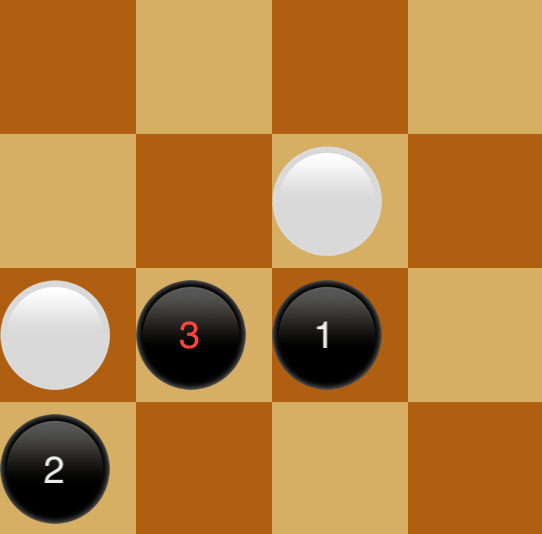
\includegraphics[scale=0.35]{images/legal_weak.png}
				\caption*{Legal weak connection}
			\end{figure}
					
			\column{0.5\textwidth}
			\begin{figure}
				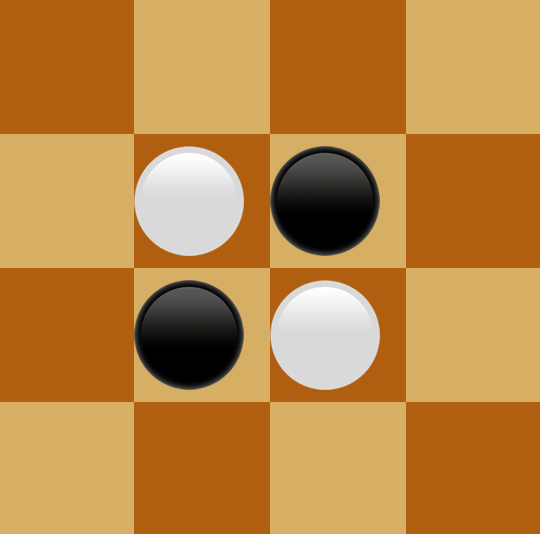
\includegraphics[scale=0.35]{images/crosscut.png}
				\caption*{Crosscut placement}
			\end{figure}
		
	\end{columns}
      \end{frame}
      
      \begin{frame}{Additional rules}
     \begin{itemize}
     \item \textbf{Pie rule}: at his first move, white can decide to switch colors with black instead of making a move.
     \item \textbf{Mandatory pass}: if a player cannot make a move (because of placement restrictions), he has to pass. It is guaranteed that at least one player can make a move.
     \end{itemize}
      \end{frame}
      
      
\section{Basic entities}
\begin{frame}{Cell}
% Lorenzo parla dei pacchetti
% inizio a parlare delle classi color, position, cell, board (diagramma uml)

\begin{columns}
\column{0.5\textwidth}
\texttt{Cell} represents the basic building block of the board 
% A cell has three fields: the position of the cell in the board, a boolean isOccupied which tells whether the cell contains a stone or not, and a Color which is the color of the stone if present.
\vspace{0.5cm}
\begin{itemize}
    \item \texttt{Position position }
    % position has two fields x,y
    \item \texttt{Color color}
    % color is an enum with two values BLACK, WHITE
    \item \texttt{boolean isOccupied}
\end{itemize}

\column{0.5\textwidth}
% uml con i tre data membri
\begin{figure}
	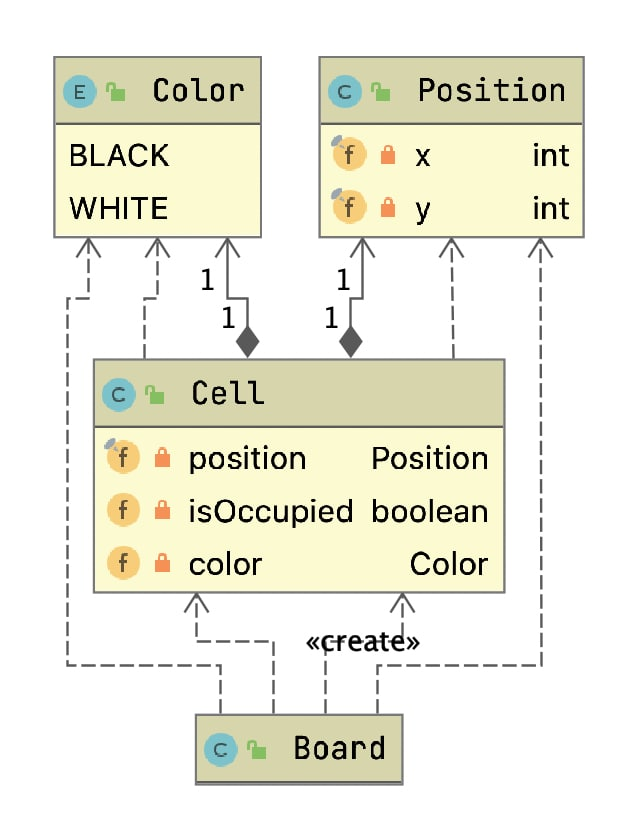
\includegraphics[scale=0.4]{images/cell-class.png}
	\caption*{Cell class}
\end{figure}

\end{columns}





\end{frame}

\begin{frame}{Cell}
	When a cell is constructed it is empty: no color is associated to it and \texttt{isOccupied=False}, when a stone is placed in the cell a color is set and \texttt{isOccupied=True}.
	
	% The methods setColor() and reset() are used for checking the rules, as we will see later. For this reason, Color is not declared as final, even if in the game once a stone is placed it cannot be moved afterwards. The position is final because a cell is associated with a fixed position in the board.

Development history:
\begin{itemize}
\item From value \texttt{NONE} in enum \texttt{Color} to field \texttt{isOccupied} in class \texttt{Cell}
\item Removed \texttt{Stone} data class
\end{itemize}
% At the beginning, the Color enum had also a NONE value, but then we thought that a Player cannot have NONE as a value for his color so we moved NONE into a new field of Cell which is a boolean called isOccupied, and the color can be only WHITE or BLACK, which is also more logical.

% at the beginning we had a class Stone but we removed it because it was a data class (only had setters, ..) and it basically coincided with Color

\end{frame}


\begin{frame}{Board}

A \texttt{Board} is represented by a set of Cells and extends \texttt{HashSet<Cell>} by overriding the \texttt{dimension()} method

Reasons for this choice of data structure:
\begin{itemize}
    \item Usage of streams
    \item \texttt{Position} as field of \texttt{Cell}    
\end{itemize}



% The board is represented by a set of cells. The other option we considered was a 2-dimensional array. In this way we can easily use streams to perform operations on this set of cells (we will see with connections). And in addition, the Position is a property (a field) of a Cell and not a pair of indexes of a matrix.

The constructor of Board creates a set of empty cells

\end{frame}





\section{Connections}
% These were the entities that make our game. Then we implemented the relationships between these entities, which are the connections, i.e. strong and weak connections between stones.

\begin{frame}{Strong connections}
\begin{itemize}
	\item We implemented a concept of orthogonal adjacency which only depends on the relative positions of two stones: the euclidean distance is 1
	\item Given the set of orthogonally adjacent stones, we implemented a method that filters only those with the same color and returns the set of strongly connected stones
\end{itemize}
	
\end{frame}

\begin{frame}{Weak connections}
\begin{itemize}
		\item Same concept used for weak connections: two stones are diagonally adjacent if their square euclidean distance is 2.	
		\item Then to obtain the set of weakly connected stones it is also necessary to filter out diagonally adjacent stones with common strong neighbors
		% in this case it is not sufficient to filter based on color 
\end{itemize}

	
\end{frame}



\section{Rules}

\begin{frame}{Rule}
	Initially, a \texttt{Rules} class was implemented to provide a way to check whether a move is valid or not and to announce whether there is a chain.
	%\\ \small From commit \href{https://github.com/lorenzobasile/konobi/blob/eaba694d6662a1b6803f7f22943636176281e572/src/main/java/konobi/Rules.java}{eaba694}
	\begin{figure}
		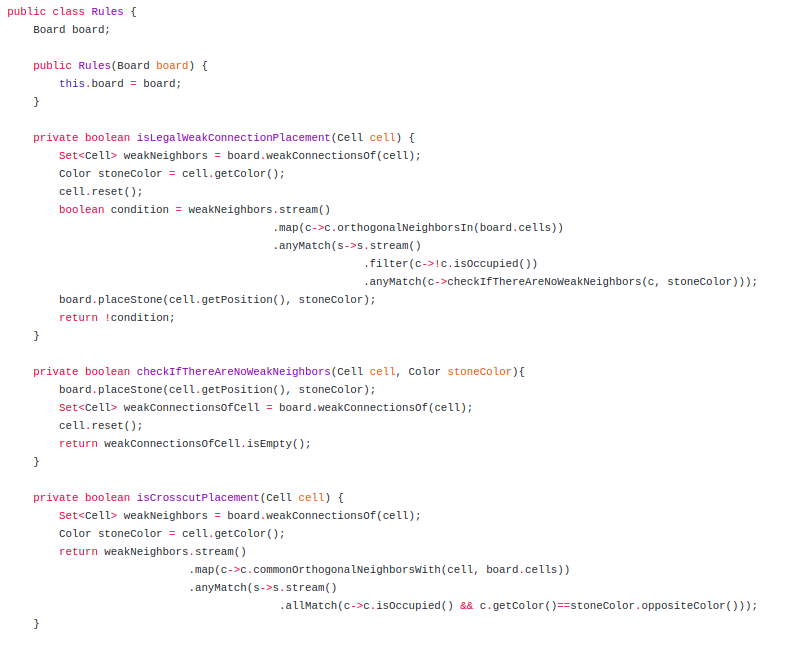
\includegraphics[scale=0.28]{images/rules-class.png}
	\end{figure}
\end{frame}

\begin{frame}{Rule}
	
	Later we realized that there would be the possibility to abstract...
	\begin{figure}
		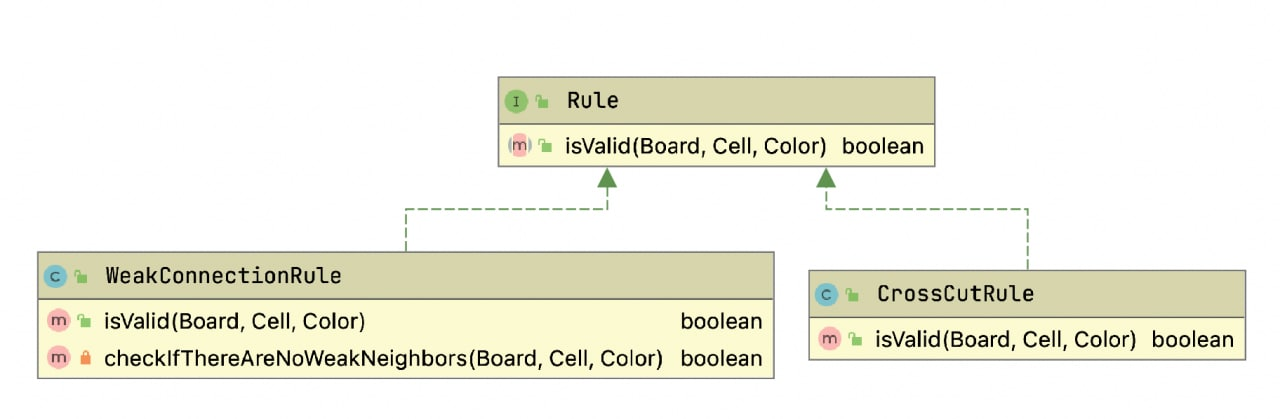
\includegraphics[scale=0.4]{images/rules-uml.jpg}
	\end{figure}

	For a given \texttt{Board}, the \texttt{isValid} method will check if it is legal to place a stone of a given \texttt{Color} in the \texttt{Cell}. \\
	\vspace{0.1cm}
	Having a \texttt{Rule} interface will allow the possibility to add new rules over the possible player's move.
	
\end{frame}

\begin{frame}{Referee}
	\begin{columns}
\column{0.5\textwidth}
	Once implemented the logic of a valid move in \texttt{Rules} package, our aim was to group together all the methods needed to check if:
	\vspace{0.4cm}
	\begin{itemize}
		\item a given move is legal w.r.t. \texttt{WeakConnectionRule} and \texttt{CrossCutRule}
		\vspace{0.25cm}
		\item a winning chain is present
		\vspace{0.25cm}
		\item the current player has to pass
	\end{itemize}
	
	\column{0.5\textwidth}
	
		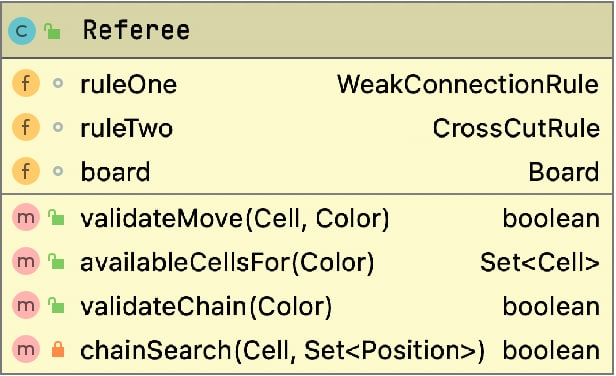
\includegraphics[scale=0.27]{images/referee-class.jpg}
	
	\end{columns}
\end{frame}



\section{InputOutput}

\begin{frame}{InputHandler and Display}
	Classes \texttt{InputHandler} and \texttt{Display} take care of game I/O.

	 \texttt{Display} contains messages to be shown to players and a method to print the board.
	
	 \texttt{InputHandler} receives inputs from player and verifies their validity using exceptions.  
\end{frame}


\section{Game dynamics}

\begin{frame}{Overview}
	  \begin{center}
     		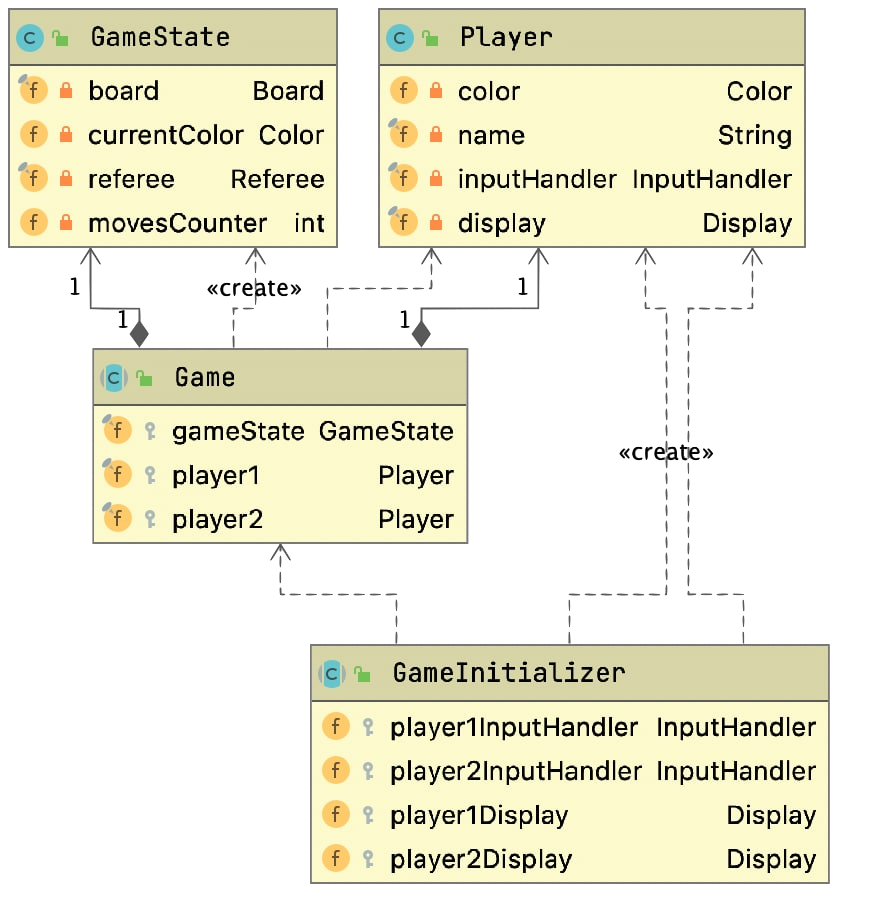
\includegraphics[scale=0.25]{images/game_uml.png}
     	\end{center}

\end{frame}

\begin{frame}{GameState}
     
     Game dynamics is managed by the \texttt{GameState} class which keeps track of current state of the game.
     \vspace{0.4cm}
     \\It is in charge of changing turn, updating the board when a valid move is received, verifying if someone has won and applying pie and pass rule.
     \vspace{0.4cm}
     \\ \texttt{GameState} acts as an intermediary between \texttt{Referee} and \texttt{Board} on one side and the higher-level class \texttt{Game} on the other 	side.
     \begin{center}
     	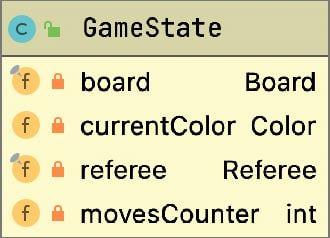
\includegraphics[scale=0.32]{images/gamestate.png}
     \end{center}
\end{frame}

\begin{frame}{Game}

	Class \texttt{Game} provides an abstraction for the game itself and instantiates a \texttt{GameState} and two players.
	
	 \texttt{Player} is defined by a color, a name, an \texttt{InputHandler} and a \texttt{Display}.
	 
	Based on the directives of \texttt{GameState}, \texttt{Game} manages the interactions with players.
\end{frame}

\begin{frame}{GameInitializer}

	\texttt{GameInitializer} abstracts the initialization of the \texttt{Game}, extended by \texttt{GameInitializerConsole} and \texttt{GameInitializerClientServer}.
	
	The initialization includes a welcome message, the construction of a \texttt{Game} and a player color message that will all be implemented in the two subclasses. 

\end{frame}

\section{Running the game}

\begin{frame}{Versions of Konobi}
INSERT UML HERE
Konobi can be played by the two players on the same terminal or in a Client-Server version, with the two players connecting through \texttt{telnet} to a Server running the game.
\end{frame}

\begin{frame}{Comparison between Console and C/S}
\begin{columns}
\column{0.5\linewidth}
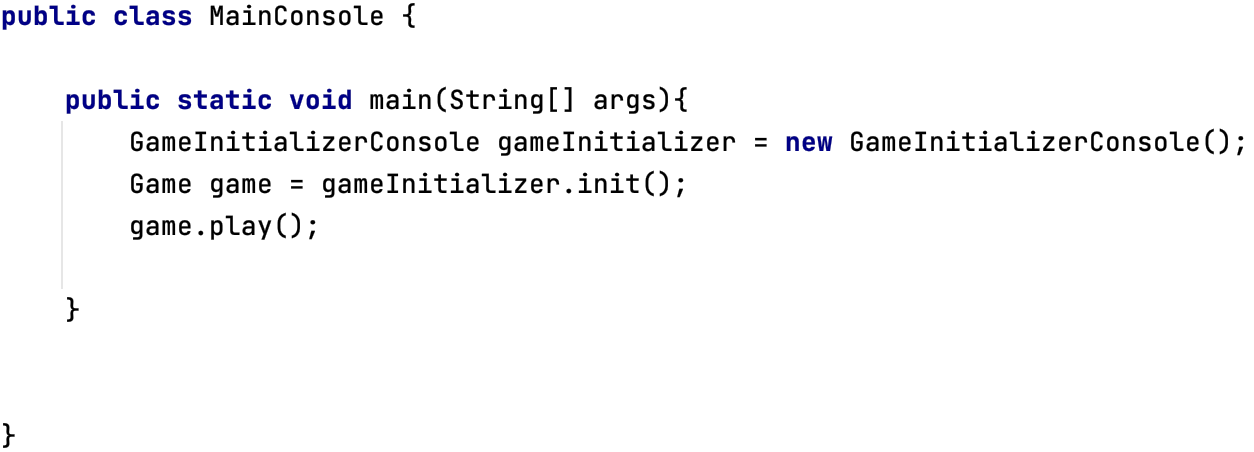
\includegraphics[scale=0.27]{images/mainCo.png}
\column{0.5\linewidth}
Console version: a \texttt{Game} is initialized and its \texttt{play} method is called.
\end{columns}
\vspace{0.5cm}
\begin{columns}
\column{0.5\linewidth}
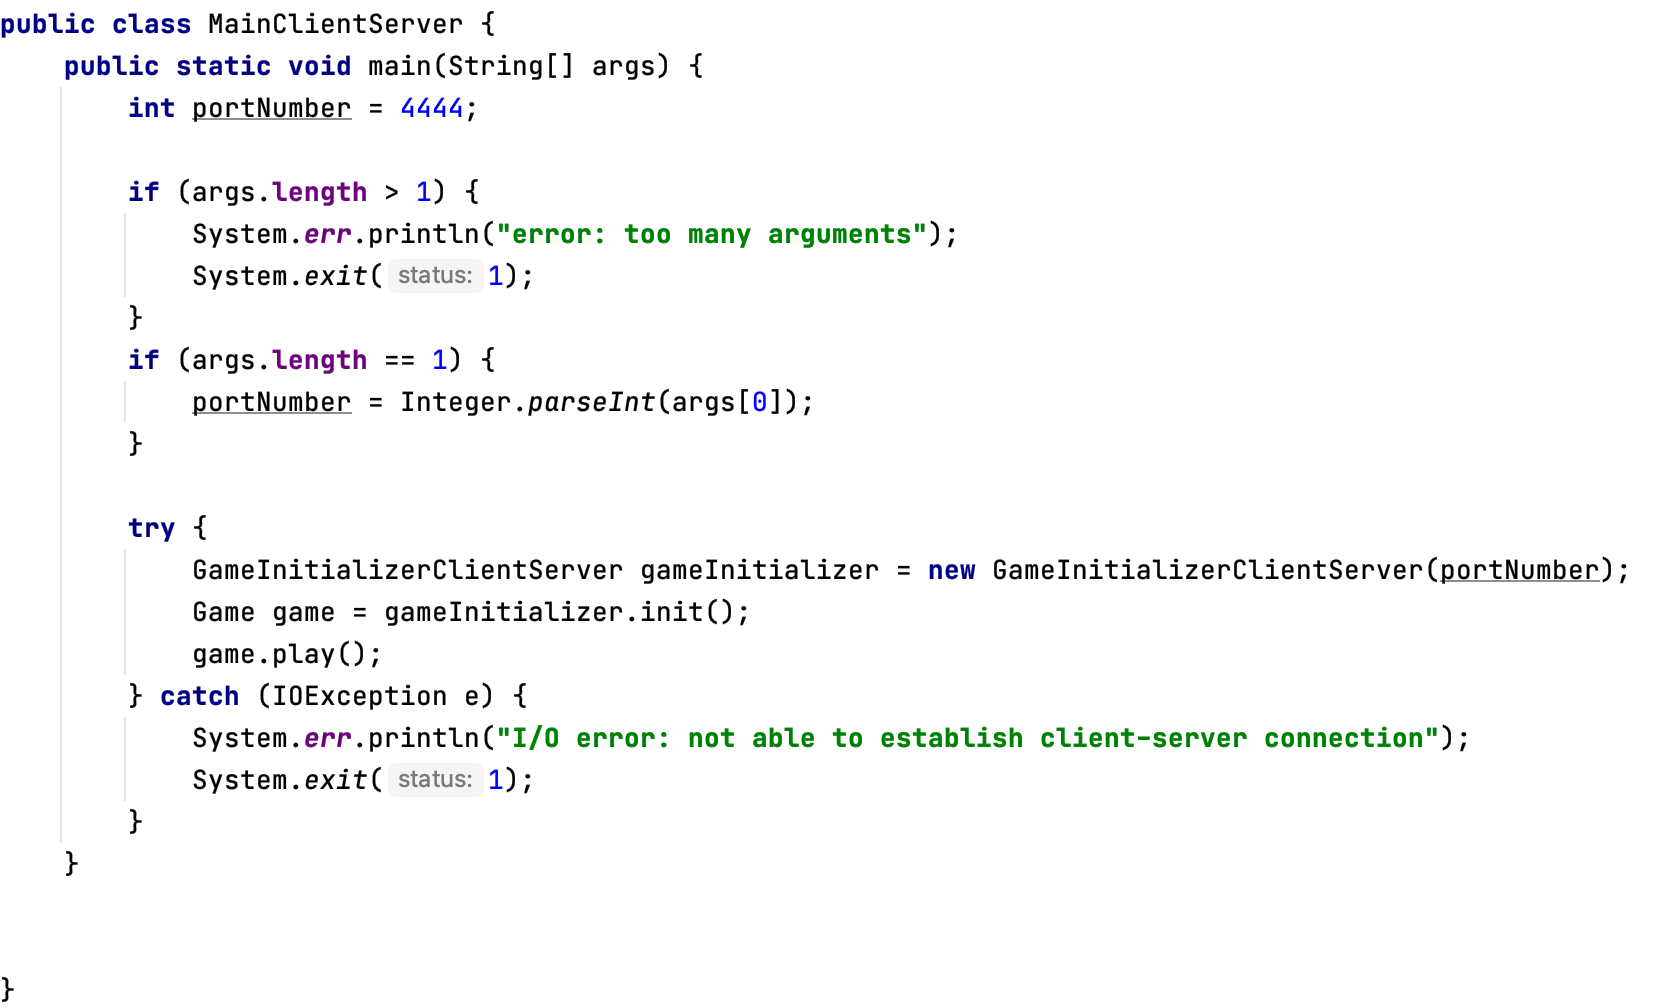
\includegraphics[scale=0.21]{images/mainCS.png}
\column{0.5\linewidth}
Client-Server version: The server creates the socket and waits for two clients to connect to it. The port number can be decided using command-line arguments.
\end{columns}\end{frame}
\begin{frame}{Inheritance in GameInitializer}

\end{frame}









     
\end{document}